\documentclass[12pt]{article}

\usepackage{epsfig}
\usepackage{rotating}
\usepackage{lscape}
\usepackage{amsfonts}
\usepackage{amssymb}
\usepackage{theorem}
\usepackage{amsmath}
\usepackage{graphicx}
%\usepackage{citesort}
\usepackage{float}
\usepackage{color}
\usepackage{array}
\usepackage{color}
\usepackage{array}
\usepackage{float}
\usepackage{url}
\usepackage{setspace}
%\usepackage{amsmath,amsfonts,amssymb,cite,array,graphicx}

\textwidth=17.36cm
\textheight=23.90cm
\hoffset=-2.37cm
\voffset=-2.5cm
\parskip=1pt

\renewcommand{\rmdefault}{ptm}

\newtheorem{definition}{Definition}[section]
\newtheorem{theorem}{Theorem}[section]
\newtheorem{corollary}{Corollary}[section]
\newtheorem{lemma}{Lemma}[section]
\newtheorem{remark}{Remark}[section]


\date{\small\today} \title{IAM851 Final Project} \author{Jeffrey Picard} 
\doublespacing

\begin{document}

\maketitle


\begin{abstract}
The purpose of this project is to gain experience with Fast Fourier Transforms (FFTs) and a commonly used FFT library called fftw by implementing an FFT
algorithm in C, in one and two dimensions, and comparing its performance to that of the existing library. Additionally this project gives an opportunity 
to use MPI by parallelizing the 2d FFT.
\end{abstract}


% main text
\section{Building and Using the Code}
The code for the project is packaged into a gzipped tarball (.tar.gz) with the use of 'make dist'. Into order to build and run the code the first step
is to unpack it with 'tar xfzv' then 'cd' into the directory and run 'autoconf -i', followed by 'configure' and then 'make' to actually build the code.
Once this is done there will be multiple executables, many used for testing the various functions that were written in the course of completing this 
project. 

The ``mpi\_alltoall\_transpose\_test'' program tests doing a matrix transpose across processes with the ``MPI\_Alltoall'' function call. Currently
this test program requires on the number of processes used be equal to $\sqrt{N}$, $N$ the number of columns in an $N by N$ matrix. The actual 
parallelized FFT does not have this stipulation.

The ``fft\_jp\_mpi\_test'' program is the original test program used in writing the parallel 2d FFT algorithm and isn't used for anything beyonf that.

The ``fftw\_test'' and ``fftw\_2d\_test'' programs use the fftw3 library to perform one and two dimensional FFTs respectively. These were the programs
used in to verify the results of the fft functions implemented for this project.

The ``fft\_jp\_test'' and ``fft\_jp\_2d\_test'' programs demonstrate how to use the code written for this project to actually perform the FFTs and
get the results. They were used to test the correctness of the fft algorithms. The ``fft\_jp\_2d\_test'' program is used to test the two different
flavors of the 2d fft function (explained in full later). When run with zero arguments it runs the first version which just outputs the result to 
a file. When run with any number of arguments it instead runs a version which returns the result of the computed fft in another argument passed to the
function.

The ``fft\_jp\_timing'' and ``fftw\_timing'' programs each take an integer argument for the number of tests that should be performed. As the
fft algorithms written for this project can only handle ffts of sizes that are powers of two, the tests will start at $2^1 = 2$ points, then $2^2=4$ points, etc
until they have all been performed. They will then output the results of the timing in a file. Figure \ref{1d_time} was created from this data.

The actual main use of the code written for this assignment is more as a few library functions rather than a program which solves an problem.
The rest of this document shall endevour to explain the use of these functions, how they were implemented and compare their performance in terms
of the fftw library and how the parallel algorithm scales with more proccessors.

\section{Output and Plots}

\begin{figure}
\begin{center}
%\includegraphics[scale=0.40]{sin.eps} 
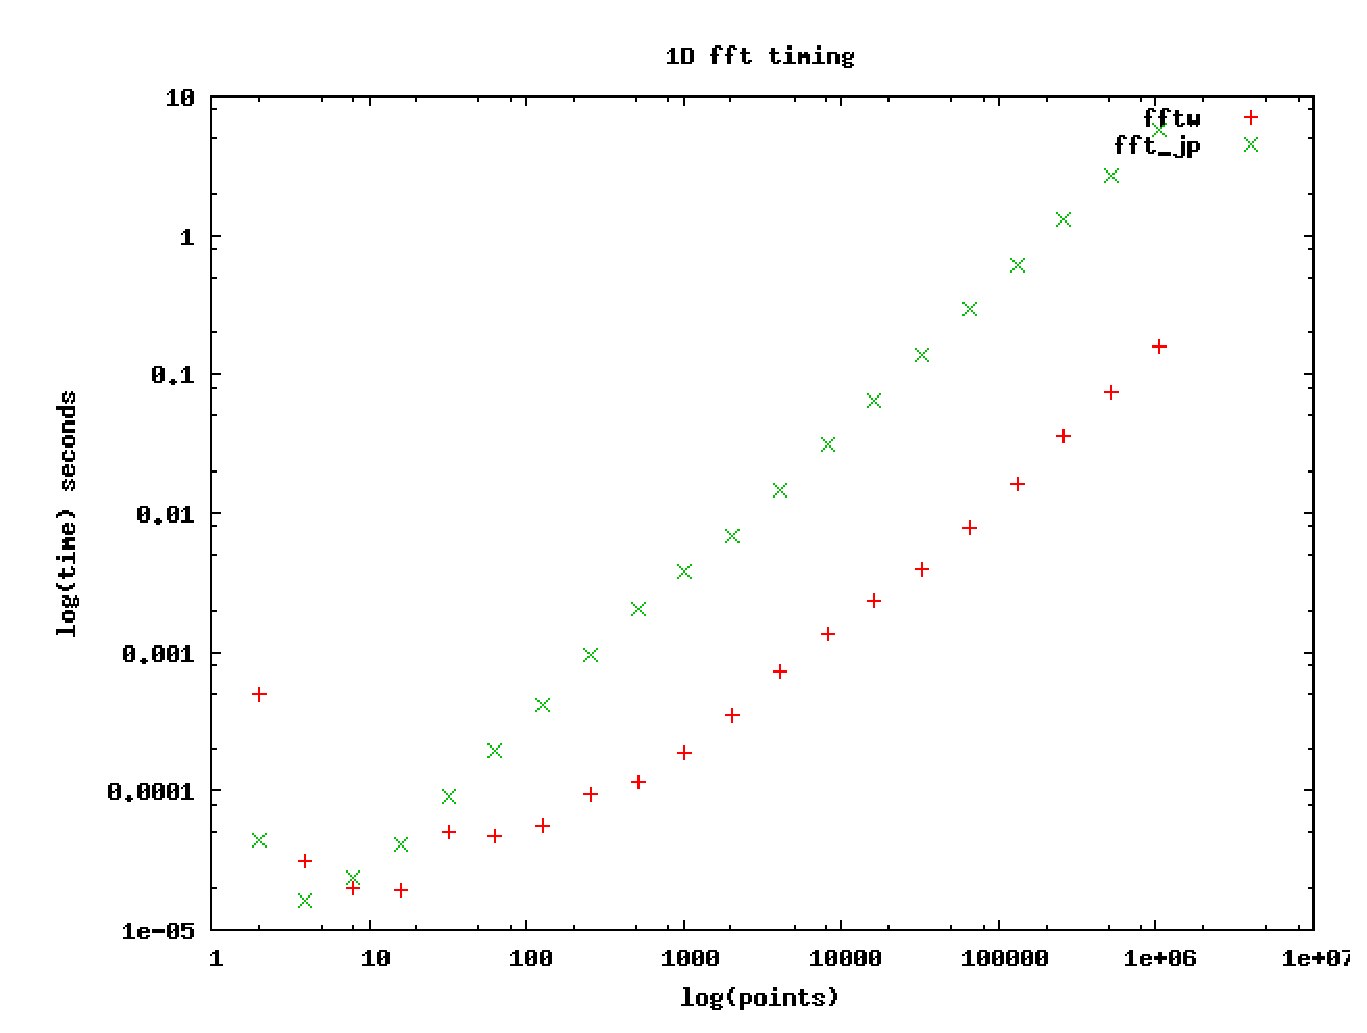
\includegraphics[scale=0.40]{figures/1d_timing.eps} \small \caption{Plot of timing for the 1d fft functions.\label{1d_time}}
\end{center}
\end{figure}


\section{Scaling with MPI}

\newpage

\section{Discussion of Code Specifics}

\end{document}
